\documentclass{emulateapj}
\submitted{{\it Submitted for publication in ApJ}}
\usepackage{multirow,color,wrapfig,ulem}
\usepackage {graphicx}
\usepackage{graphics}
\usepackage[dvips]{epsfig}

%=========================================================================
%		INTERNAL MACROS
%=========================================================================
\def\be{\begin{equation}}
\def\ee{\end{equation}}
\def\ba{\begin{eqnarray}}
\def\ea{\end{eqnarray}}

% To highlight comments 
\definecolor{red}{rgb}{1,0.0,0.0}
\newcommand{\red}{\color{red}}
\definecolor{darkgreen}{rgb}{0.0,0.5,0.0}
\newcommand{\SRK}[1]{\textcolor{darkgreen}{\bf SRK: \textit{#1}}}
\newcommand{\SRKED}[1]{\textcolor{darkgreen}{\bf #1}}
\newcommand{\before}[1]{\textcolor{red}{ #1}}
\newcommand{\after}[1]{\textcolor{darkgreen}{ #1}}

\newcommand{\LCDM}{$\Lambda$CDM~}
\newcommand{\beq}{\begin{eqnarray}}  
\newcommand{\eeq}{\end{eqnarray}}  
\newcommand{\zz}{$z\sim 3$} 
\newcommand{\avg}[1]{\langle{#1}\rangle}  
\newcommand{\ly}{{\ifmmode{{\rm Ly}\alpha}\else{Ly$\alpha$}\fi}}
\newcommand{\hMpc}{{\ifmmode{h^{-1}{\rm Mpc}}\else{$h^{-1}$Mpc}\fi}}  
\newcommand{\hGpc}{{\ifmmode{h^{-1}{\rm Gpc}}\else{$h^{-1}$Gpc}\fi}}  
\newcommand{\hmpc}{{\ifmmode{h^{-1}{\rm Mpc}}\else{$h^{-1}$Mpc}\fi}}  
\newcommand{\hkpc}{{\ifmmode{h^{-1}{\rm kpc}}\else{$h^{-1}$kpc}\fi}}  
\newcommand{\hMsun}{{\ifmmode{h^{-1}{\rm {M_{\odot}}}}\else{$h^{-1}{\rm{M_{\odot}}}$}\fi}}  
\newcommand{\Mmin}{{\ifmmode{{M_{\rm min}}}\else{${M_{\rm min}}$}\fi}}
\newcommand{\mmin}{{\ifmmode{{M_{\rm min}}}\else{${M_{\rm min}}$}\fi}}
\newcommand{\mmax}{{\ifmmode{{M_{\rm max}}}\else{${M_{\rm max}}$}\fi}}
\newcommand{\lmmin}{{\ifmmode{{\log M_{\rm min}}}\else{${\log M_{\rm min}}$}\fi}}
\newcommand{\lmmax}{{\ifmmode{{\log M_{\rm max}}}\else{${\log M_{\rm max}}$}\fi}}

\newcommand{\Mmax}{{\ifmmode{{M_{\rm max}}}\else{${M_{\rm max}}$}\fi}}
\newcommand{\dm}{{\ifmmode{{\Delta M}}\else{$\Delta M$}\fi}}
\newcommand{\dlm}{{\ifmmode{{\Delta \log M}}\else{$\Delta \log M$}\fi}}
\newcommand{\focc}{{\ifmmode{{f_{\rm occ}}}\else{${f_{\rm occ}}$}\fi}}

\newcommand{\Msun}{{\ifmmode{{\rm {M_{\odot}}}}\else{${\rm{M_{\odot}}}$}\fi}}  
\newcommand{\msun}{{\ifmmode{{\rm {M_{\odot}}}}\else{${\rm{M_{\odot}}}$}\fi}}  
\newcommand{\lya}{{Lyman$\alpha$~}}
\newcommand{\clara}{{\texttt{CLARA}}~}
\newcommand{\rand}{{\ifmmode{{\mathcal{R}}}\else{${\mathcal{R}}$ }\fi}}  
%SAMPLES


%MY COMMANDS #############################################################
\newcommand{\sub}[1]{\mbox{\scriptsize{#1}}}
\newcommand{\dtot}[2]{ \frac{ d #1 }{d #2} }
\newcommand{\dpar}[2]{ \frac{ \partial #1 }{\partial #2} }
\newcommand{\pr}[1]{ \left( #1 \right) }
\newcommand{\corc}[1]{ \left[ #1 \right] }
\newcommand{\lla}[1]{ \left\{ #1 \right\} }
\newcommand{\bds}[1]{\boldsymbol{ #1 }}
\newcommand{\oiint}{\displaystyle\bigcirc\!\!\!\!\!\!\!\!\int\!\!\!\!\!\int}
\newcommand{\mathsize}[2]{\mbox{\fontsize{#1}{#1}\selectfont $#2$}}
\newcommand{\eq}[2]{\begin{equation} \label{eq:#1} #2 \end{equation}}
\newcommand{\lth}{$\lambda_{th}$ }
\newcommand{\reff}{{\ifmmode{r_{\mbox{\tiny eff}}}\else{$r_{\mbox{\tiny eff}}$}\fi}}
%#########################################################################

%TO DO COMMANDS. Highlight region that needs extra work  #############################################################
\newcommand{\todo}{\ifmmode \text{\Huge{\(\bullet\)}} \else {\Huge$\bullet$}\fi}
% \newcommand{\todo}{\ifmmode {\Huge \bullet} \else {\Huge$\bullet$}\fi}
\newcommand{\tido}{\ifmmode {\bullet} \else $\bullet$\fi}
\newcommand{\REFS}{(\todo REFS) }
\newcommand{\toref}{(\todo REFS)}
%#########################################################################



\begin{document}
%=========================================================================
%		FRONT MATTER
%=========================================================================
\title{Local Group Satellite Alignments in a Cosmological Context: Insights from the Illustris Simulation}
\author{
  Ver\'onica Arias \thanks{v.arias@uniandes.edu.co}$^{1}$,
  Jaime E. Forero-Romero \thanks{je.forero@uniandes.edu.co}$^{2}$ 
}

\affil{
$^1$Departamento de F\'{i}sica, Universidad de los Andes, Cra. 1
No. 18A-10, Edificio Ip, Bogot\'a, Colombia\\
}




\begin{abstract}
Alineaciones.
\end{abstract}

\keywords{
Galaxies: halos --- Galaxies: high-redshift --- Galaxies: statistics
--- Dark Matter --- Methods: numerical 
}

\section{Introduction}

Observational evidence of planes is everywhere (where we can see them). MW, M31, Centaurus A.\\

Not so evident in simulations:\\

Millenium II Baumgardt, Ibata, Pawlowski\\

Clues Gillet está pero diferente\\

Plane claims:\\
Libeskind: preferential direction for accretion.\\
Sawala: planes are there when baryonic physics is included.\\
Buck: planes are easy to form at early times, when DM filaments are very thin. In high redshift galaxies galaxies, planes are everywhere.\\

Other explanations: Kroupa: tidal dwarfs\\
Fouquet\\



 
Following a bit on the claim by Sawala that barionic physics are important when looking for planes, WE look in Illustris and Elvis simulations to try and understand why barionic physics results in planar distribution of satellites.

\section{Sample Selection}

\begin{figure}
\centering
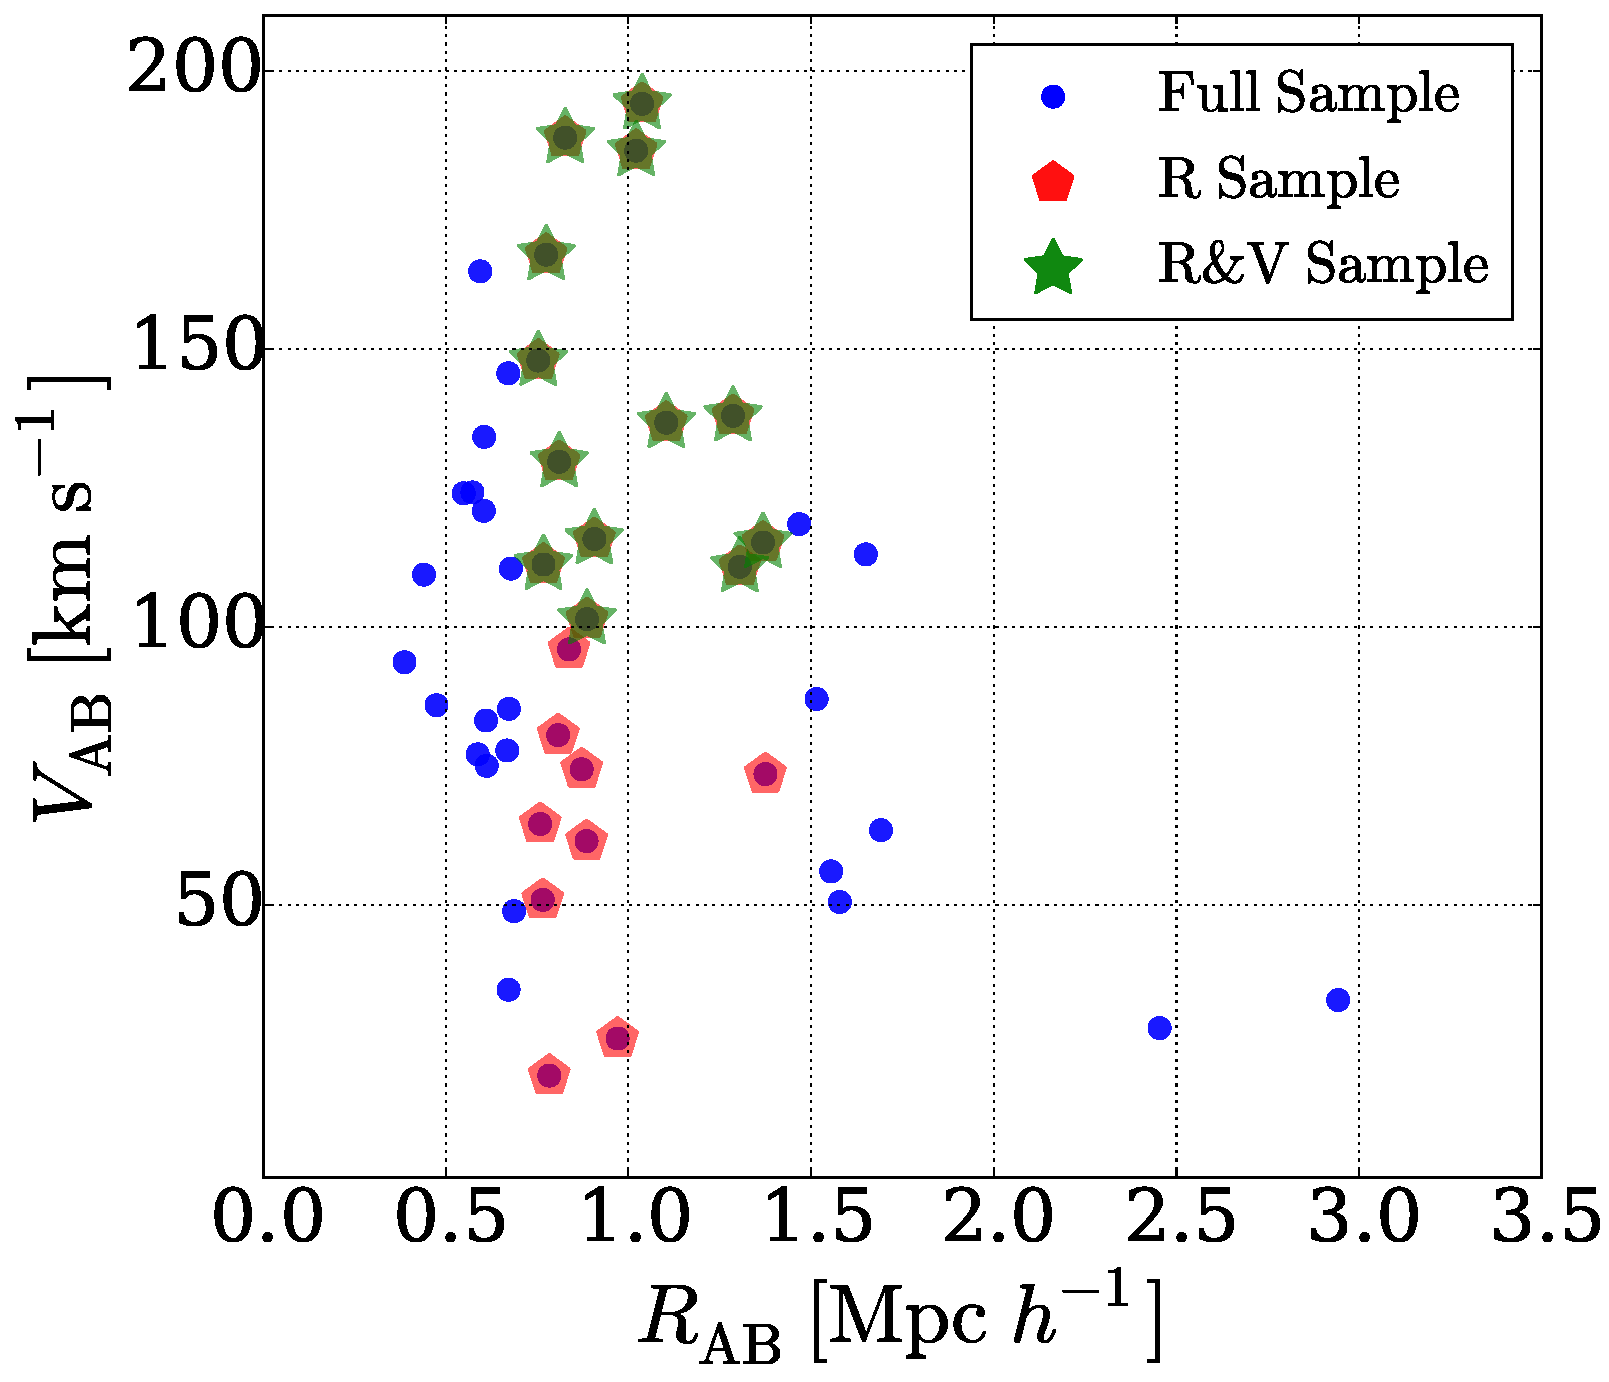
\includegraphics[width=\hsize]{v_r_pairs.pdf}\\
\caption{Halo pair samples used in this paper located in the
  plane of relative comoving velocity $V_{AB}$ versus relative
  distance $R_{AB}$ between the two halos in the pair.
  The R\&V sample is the closest to the separation and kinematic
  conditions observed in the Local Group.} 
\label{fig:samples}
\end{figure}

\begin{figure}
\centering
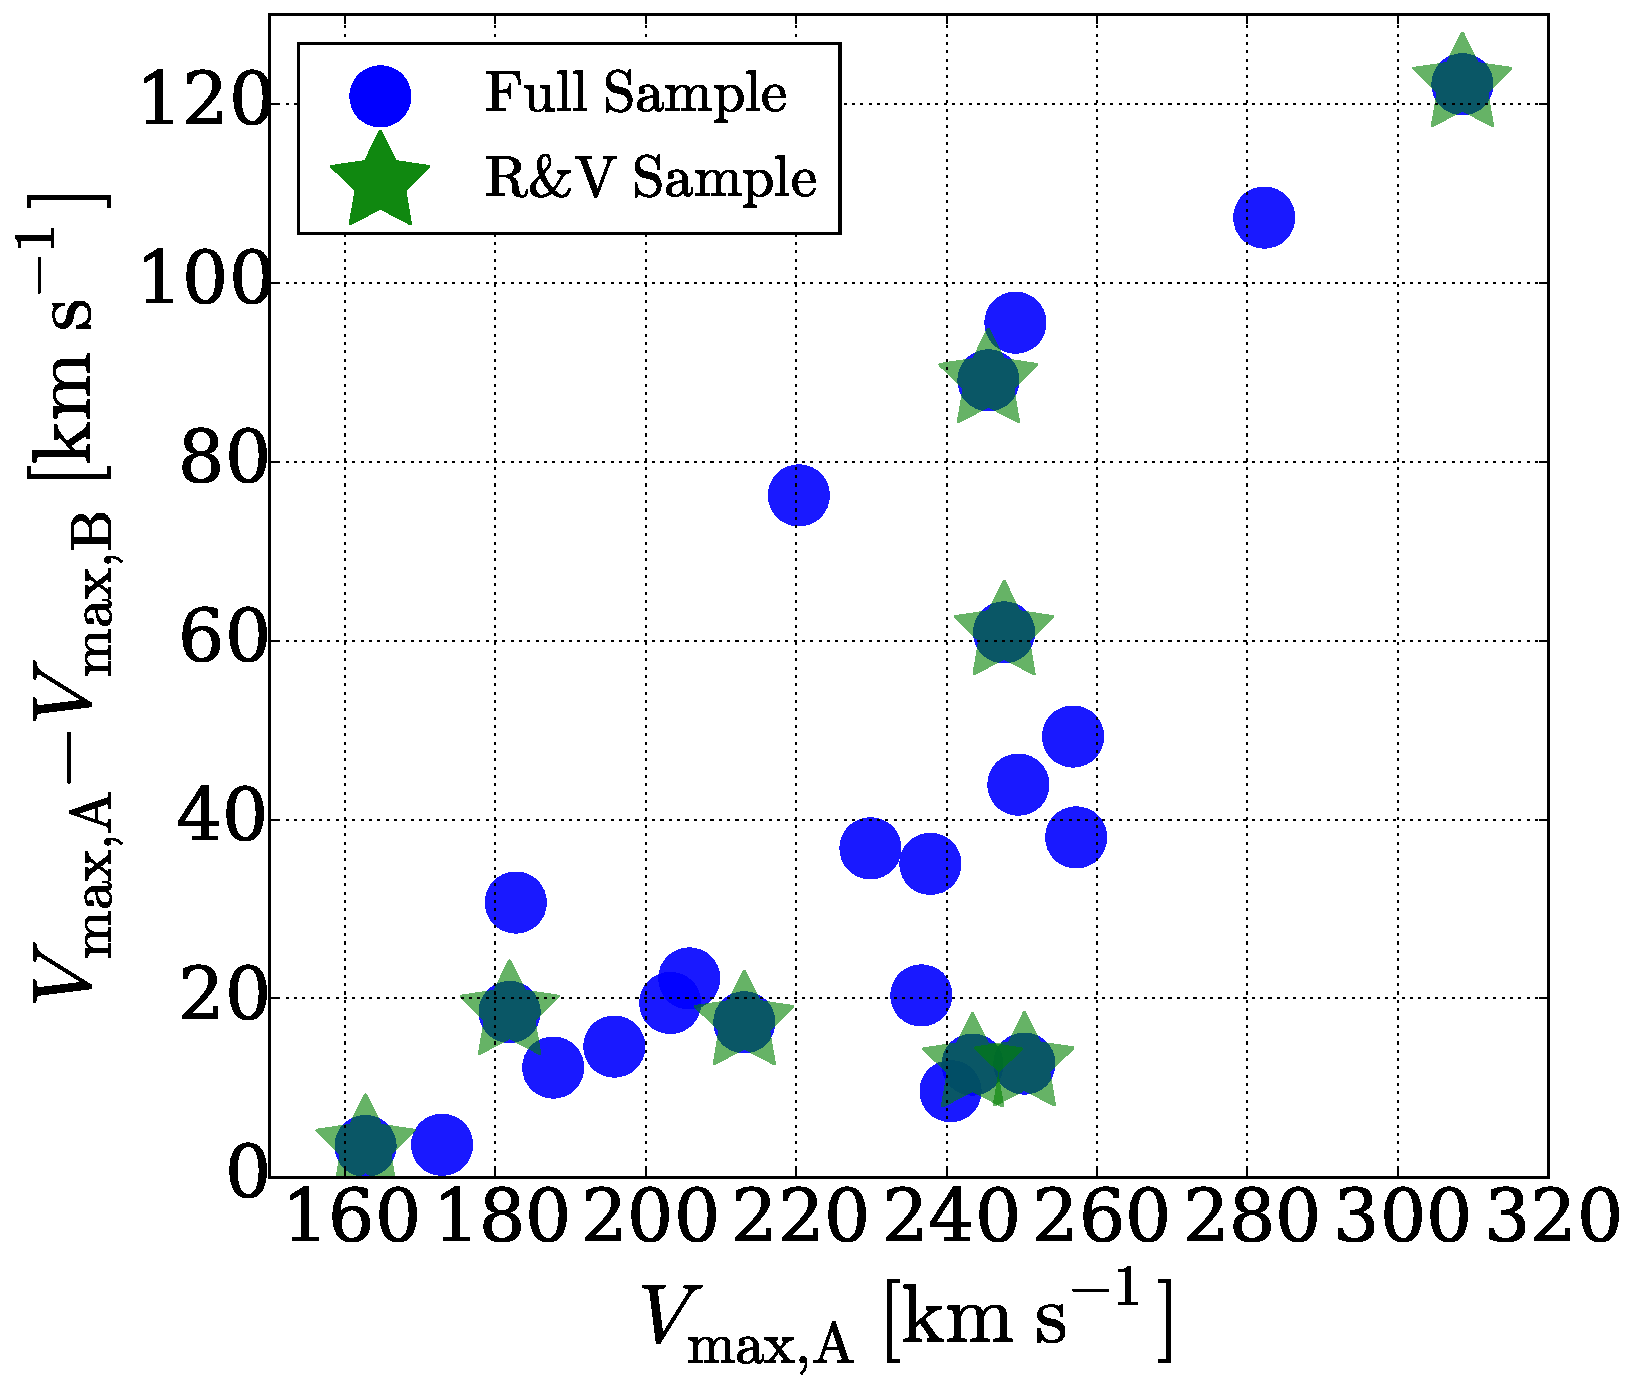
\includegraphics[width=\hsize]{v_circ_pairs.pdf}\\
\caption{Diference between the maximum circular velocity $V_{max}$ for the two
  halos in the pair as a function of $V_{max}$ for the massive halo in
  the pair.}
\label{fig:vcirc}
\end{figure}

\begin{figure}
\centering
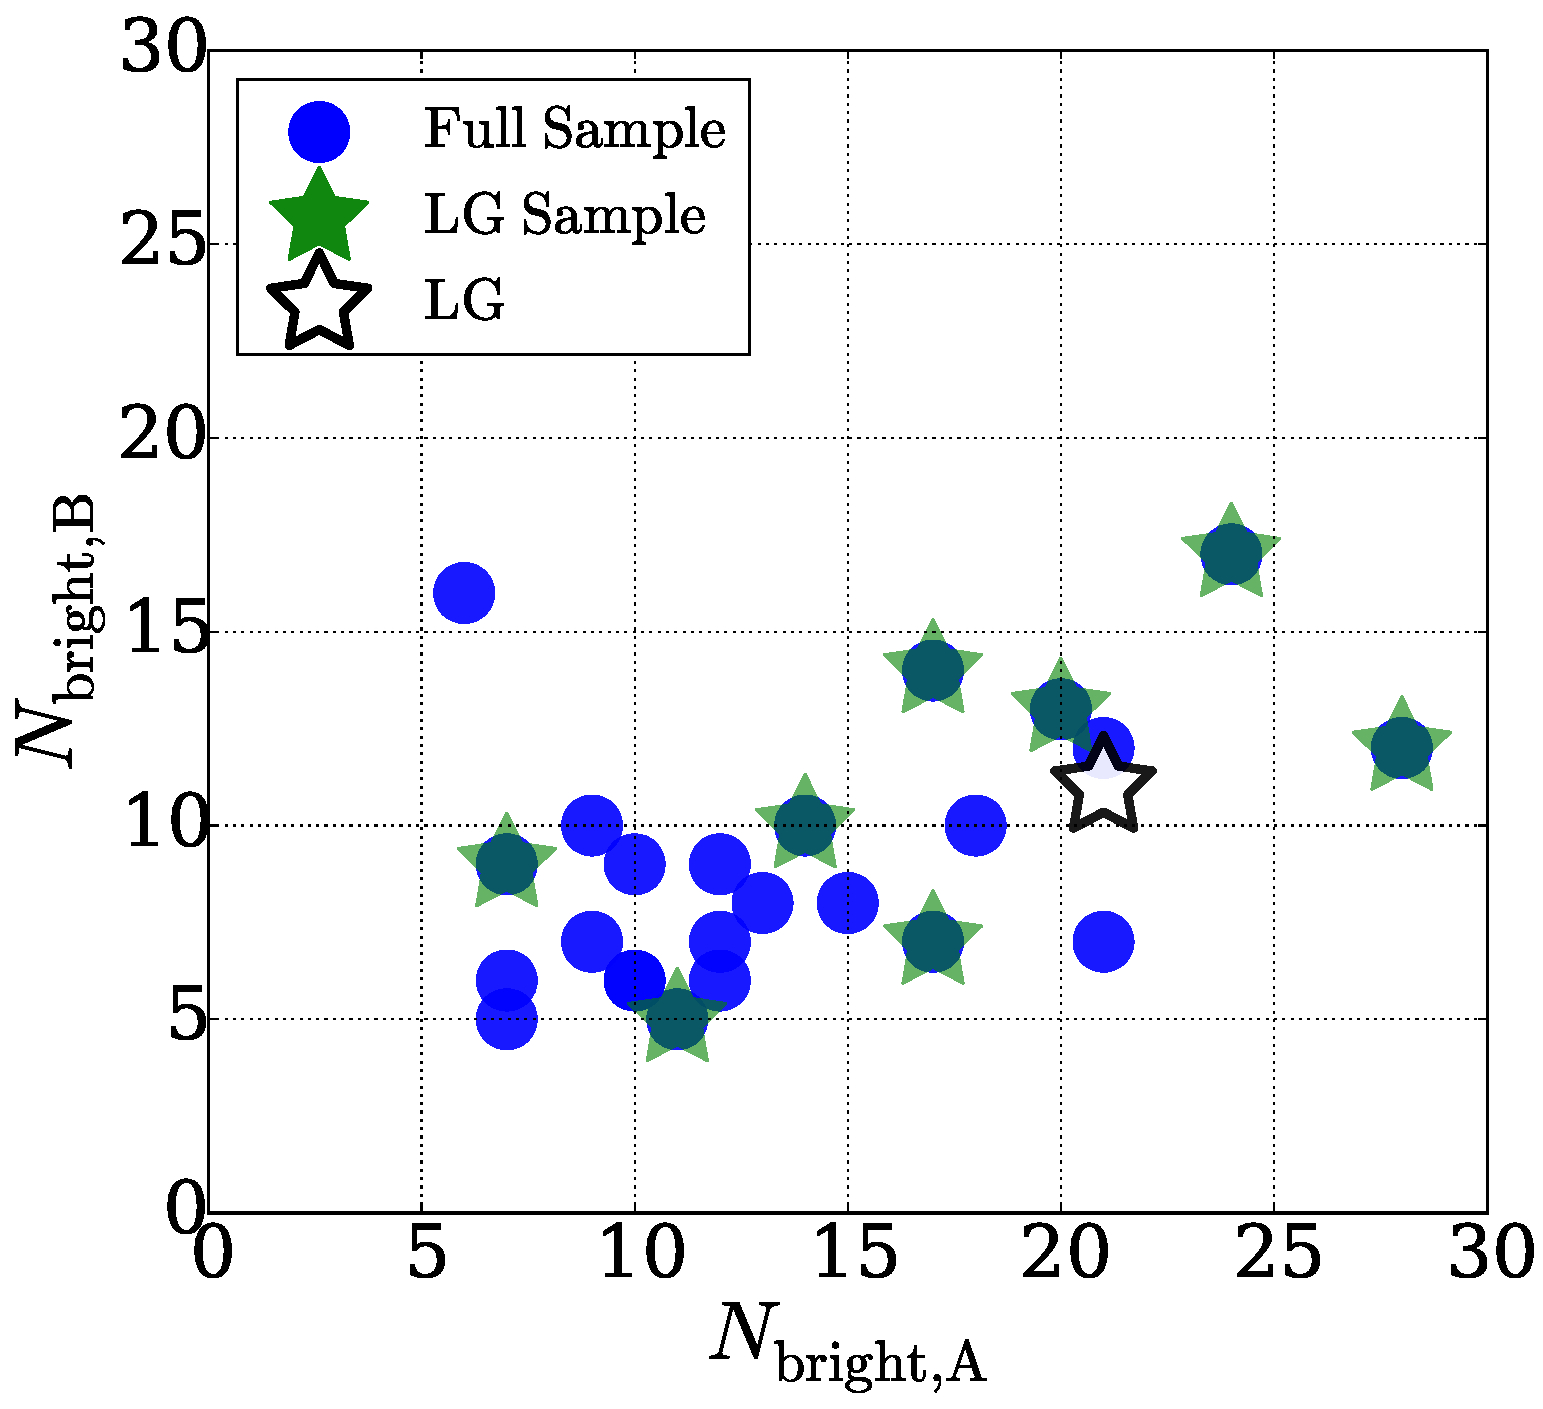
\includegraphics[width=\hsize]{n_structure.pdf}\\
\caption{Number of bright substructures ($M_{B}<-9$) and dark matter
  substructures.}
\label{fig:nstructure}
\end{figure}



\begin{figure}
\centering
\includegraphics[width=\hsize]{axratio_dark_bright.pdf}\\
\caption{Axis ratio of luminous satellites versus the axis ratio for
  dark subhalos.}
\label{fig:StreamPlaneOrbit}
\end{figure}


\begin{figure*}
\centering
\includegraphics[width=0.48\hsize]{significance_full_dark.pdf}
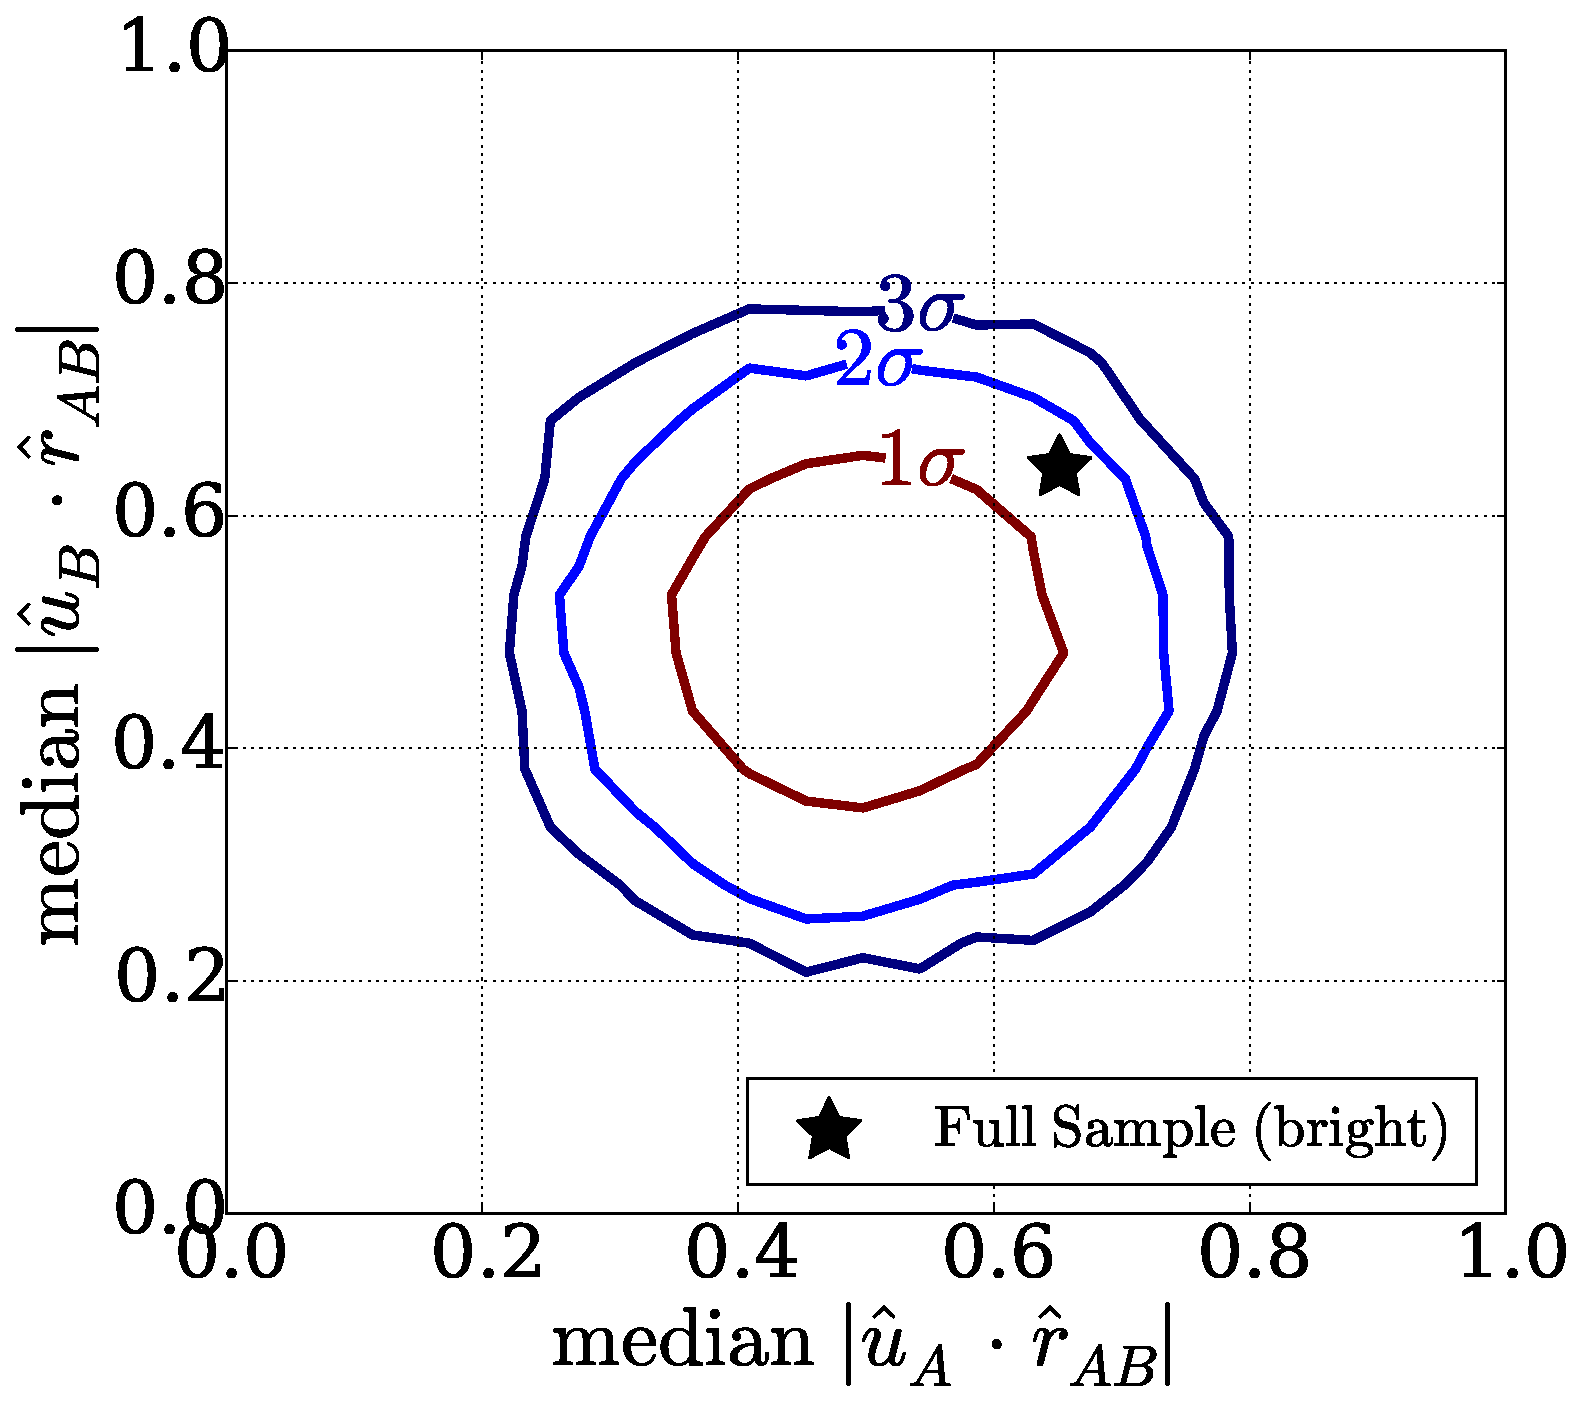
\includegraphics[width=0.48\hsize]{significance_full_bright.pdf}\\
\includegraphics[width=0.48\hsize]{significance_lg_dark.pdf}
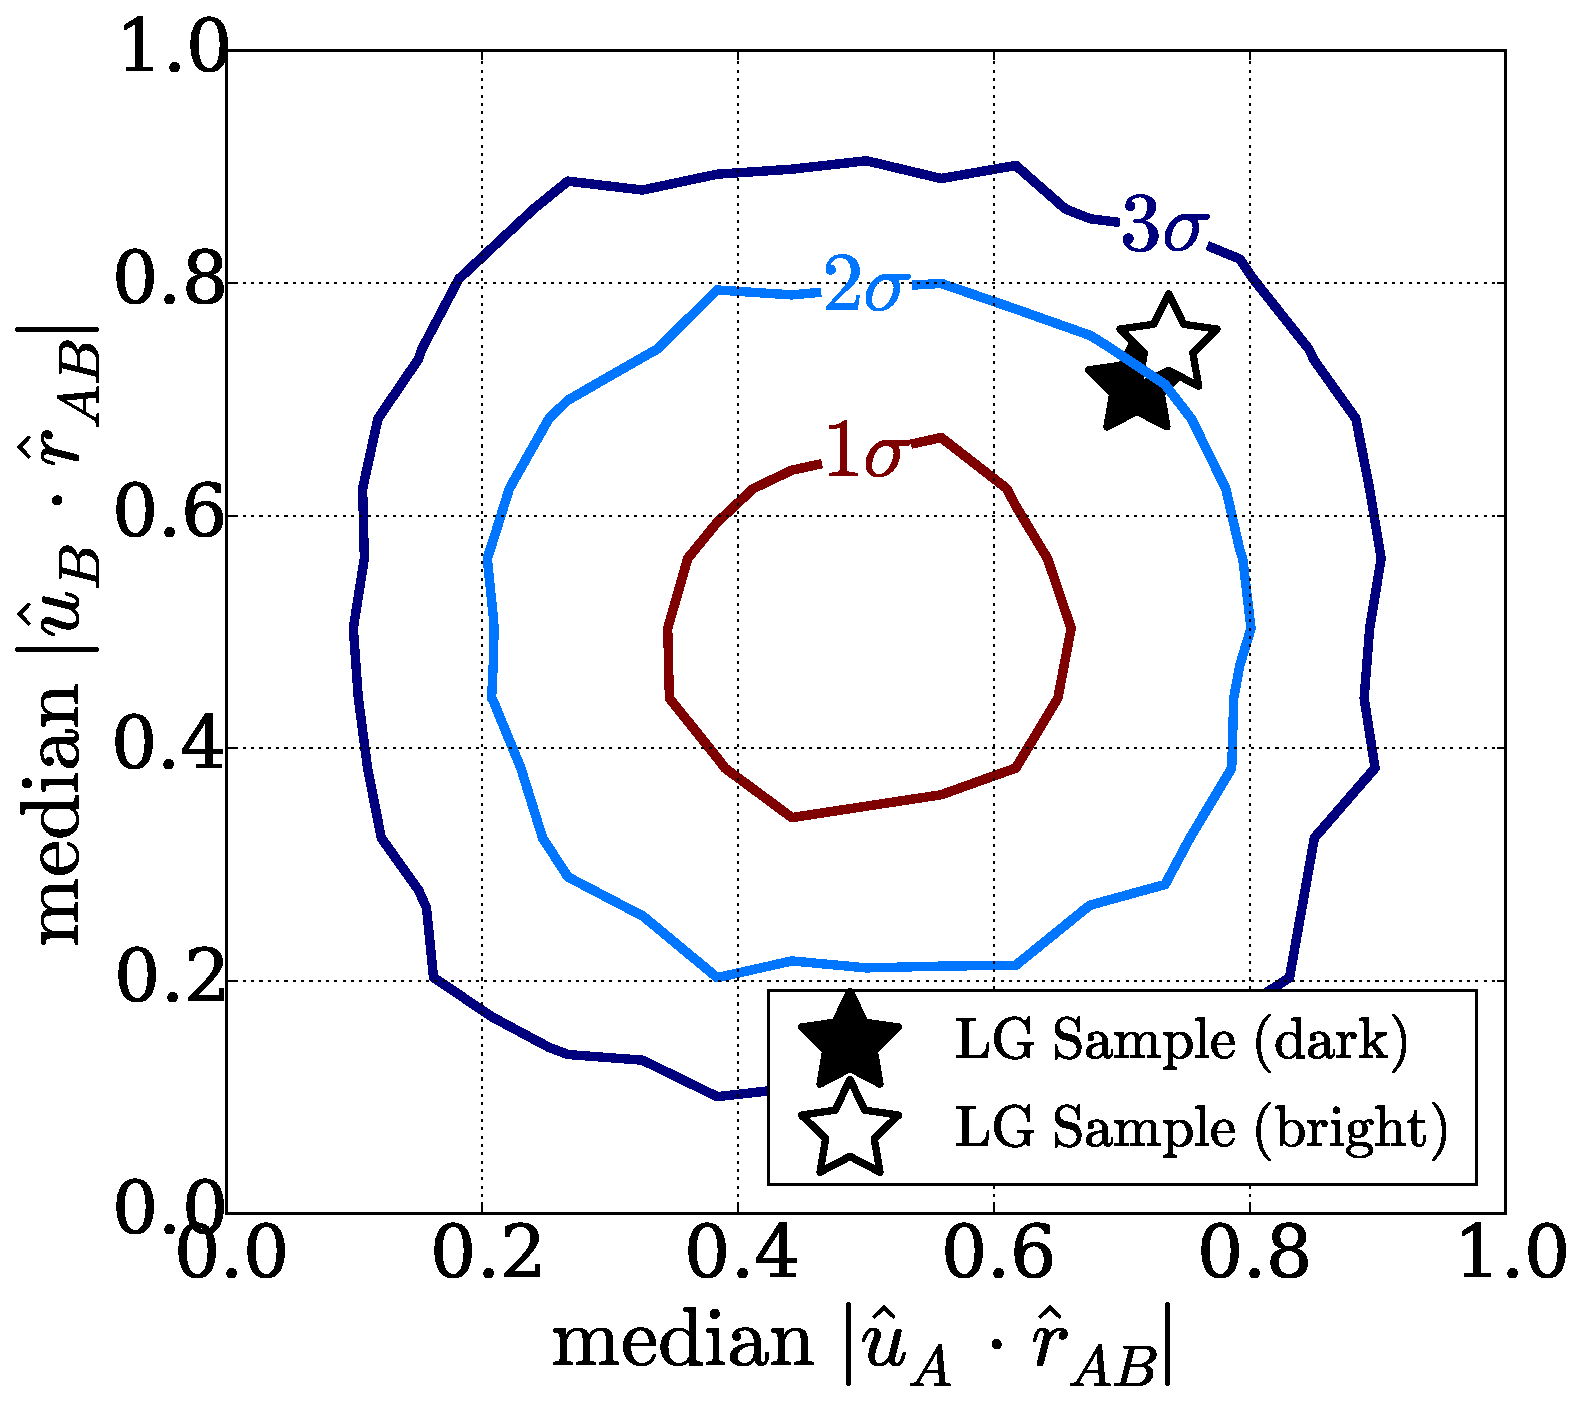
\includegraphics[width=0.48\hsize]{significance_lg_bright.pdf}\\
\caption{Significance of alignments.}
\label{fig:significance}
\end{figure*}

\begin{figure}
\centering
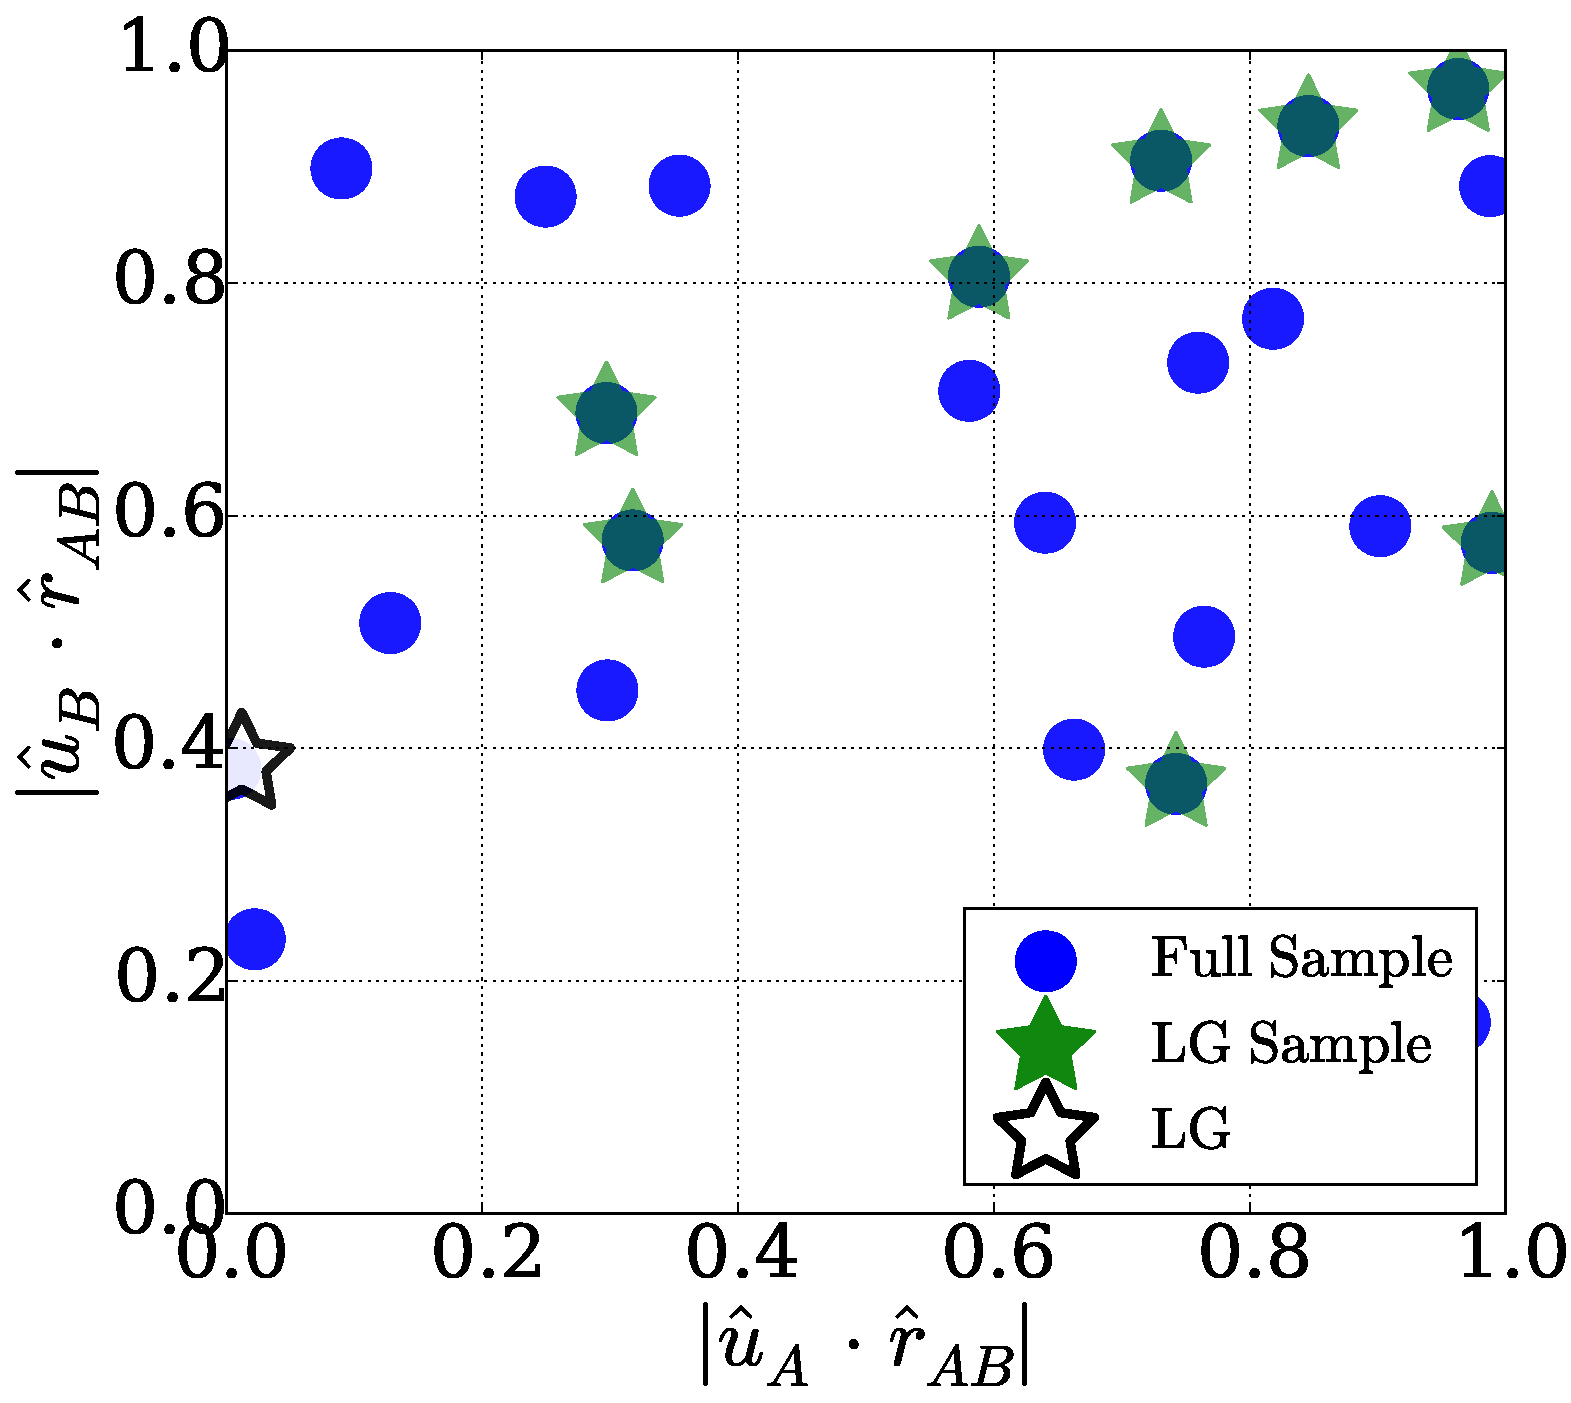
\includegraphics[width=\hsize]{r_u_alignment.pdf}\\
\caption{Alignment of the mayor axis with the vector connecting the
  two halos.}
\label{fig:lg_alignment}
\end{figure}

\begin{figure}
\centering
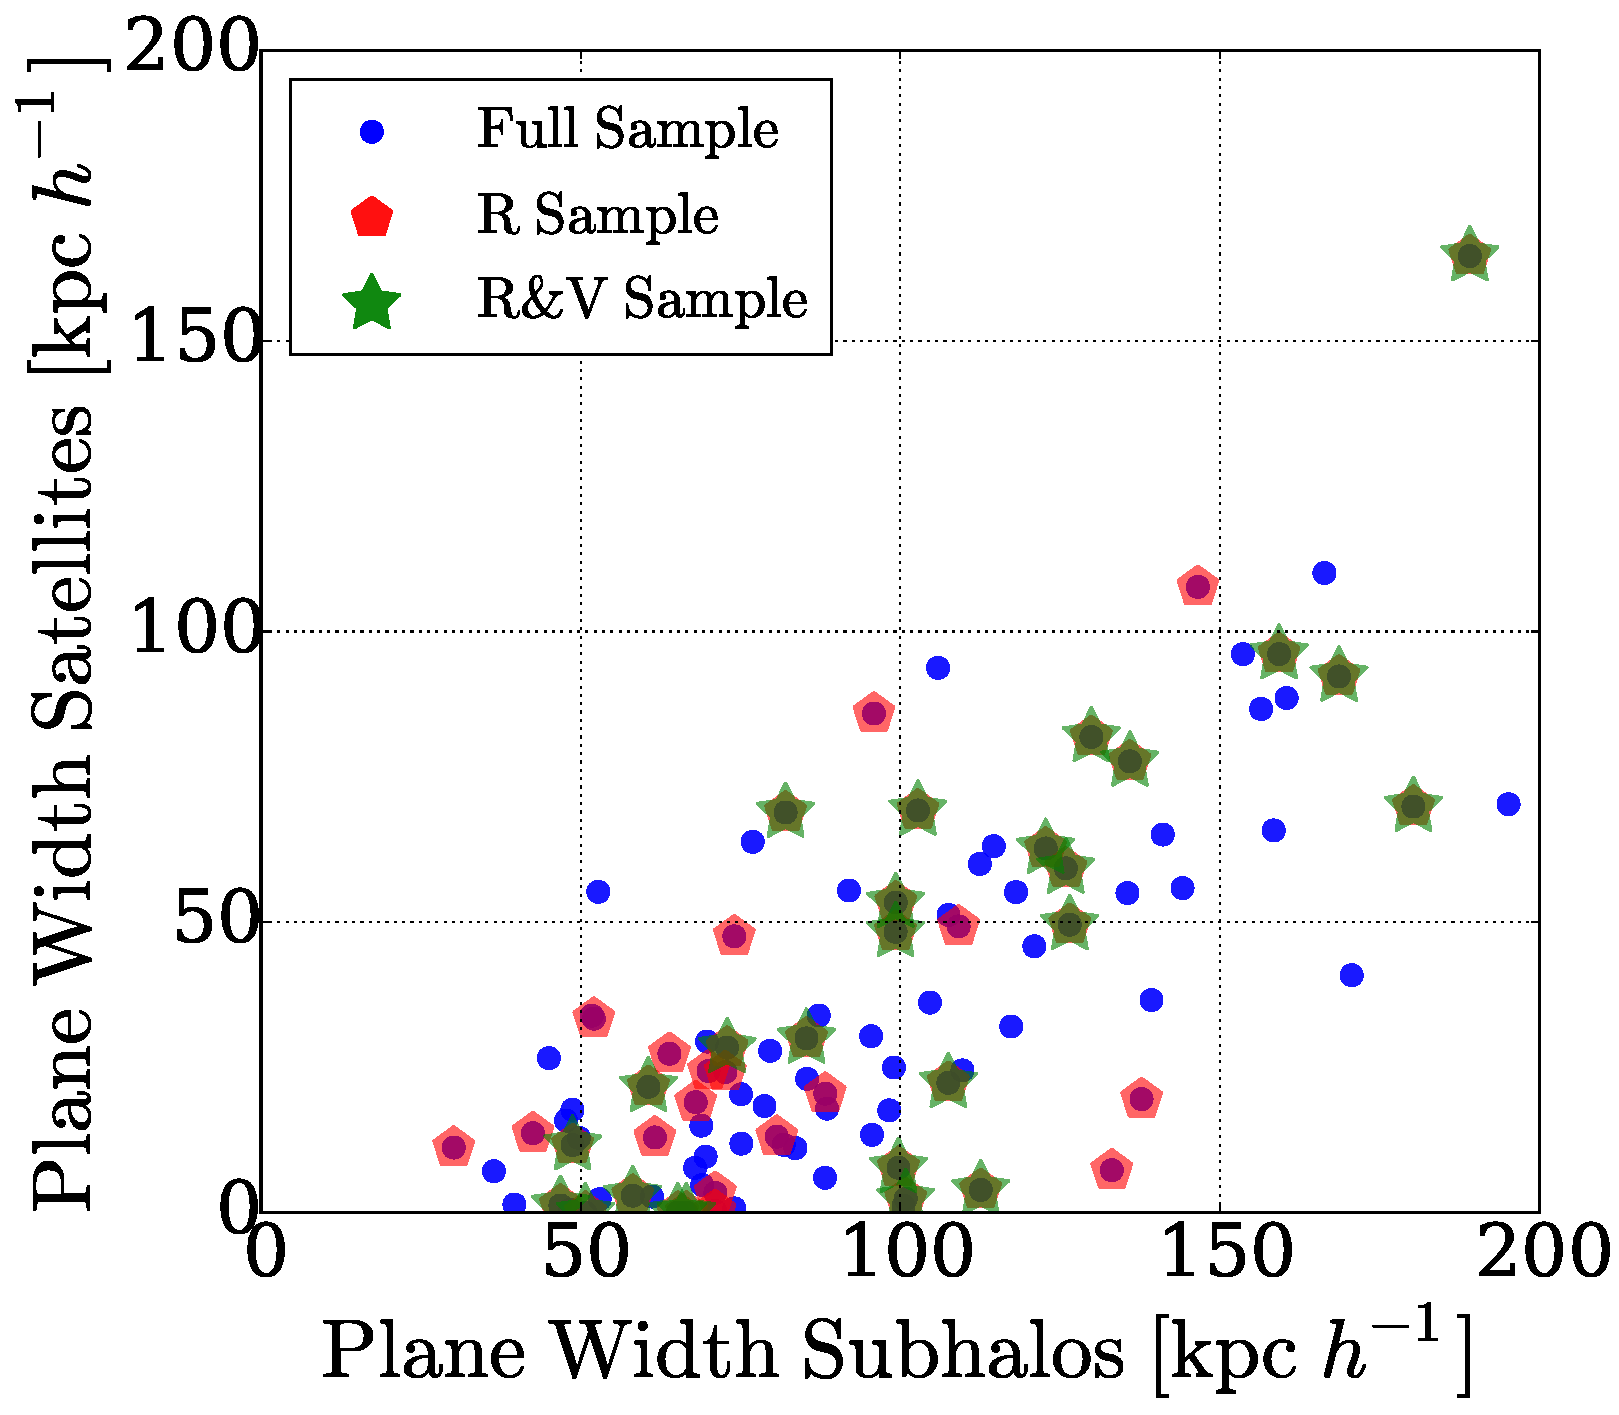
\includegraphics[width=\hsize]{plane_width.pdf}\\
\caption{Plane width for the best planes in the luminious and dark cases.}
\label{fig:plane_width}
\end{figure}

\begin{figure}
\centering
\includegraphics[width=\hsize]{plane_width_n_dark.pdf}\\
\caption{Plane width as a function of objects used to find the plane.}
\label{fig:plane_width_nobjects}
\end{figure}

\section{Results}
\label{Results}

\section{Method}
\label{Method}



%\begin{figure}
%\centering
%\includegraphics[width=\hsize]{Halo_pos_LRomulusRemus.pdf}\\
%\end{figure}

\section{Discussion} 
\section{Acknowledgements}
Gracias.
\bibliographystyle{apj}
\bibliography{Dwarfs}


\end{document}

